\documentclass[a4paper]{article}

\usepackage[utf8]{inputenc}
\usepackage[spanish]{babel}
\usepackage[margin=2cm, top=2cm, includefoot]{geometry}%--para definir espacio de márgenes
\usepackage{graphicx}%--para insertar imágenes
\usepackage{fancyhdr}%--para el estilo con barra arriba de las páginas
\usepackage[table,xcdraw]{xcolor}%--para la detección de colores
\usepackage[hidelinks]{hyperref}%--para hipervínculos
\usepackage{parskip}%--para evitar tabulación de inicio de párrafo
\usepackage{booktabs}%--
\usepackage{multirow, array}
\usepackage{ragged2e}
\usepackage{float}

%definiendo color
\definecolor{rojoOscuro}{HTML}{A20303}
%---definiendo estilo del informe
\setlength{\headheight}{56.10185pt}
\pagestyle{fancy}
\fancyhf{}
\lhead{\hspace{0.1cm} 
\includegraphics[height=1.55cm]{imagenes/CiberSecFIIS.png}}\rhead{
\includegraphics[height=1.5cm]{imagenes/uni_logo.png} \hspace{0.1cm}}

%---Cambios
\renewcommand{\headrulewidth}{3pt}%--grosor de la linea superior
\renewcommand{\headrule}{\hbox to\headwidth{\color{rojoOscuro}\leaders\hrule height \headrulewidth\hfill}}%--definir la linea base superior
\renewcommand{\arraystretch}{2}%--espaciado de las tablas
%---Inicio de informe

\begin{document}
    \begin{titlepage}
    \centering
        {\large \textbf{UNIVERSIDAD NACIONAL DE INGENIERÍA}} \par \vspace{0.3cm}
        {\large \textbf{FACULTAD DE INGENIERÍA INDUSTRIAL Y DE SISTEMAS}} \par \vspace{1.125cm}
        
\includegraphics[width=0.7\textwidth]{imagenes/CiberSecFIIS.png} \par \vspace{1.125cm}
        {\LARGE \textbf{Segunda Evaluación de Penetración de Seguridad}}\par \vspace{1cm}
        {\Large \textbf{Elaborado por:}} \par \vspace{1cm}
        \vfill
        {\large \textbf{Carolina Aliaga}} \par \vspace{0.8cm}
        {\large \textbf{Elian Paucar}} \par \vspace{3.55cm}
        \vfill
        {\textbf{Lima, 2021}}
\end{titlepage}

%-----------------------------------------------------------
    \clearpage
        \tableofcontents
    \clearpage
%------------------------------------------------------------
    \listoffigures
    \clearpage
%------------------------------------------------
    %----Para el inicio de numeración a partir de aquí---
    \cfoot{\thepage}
    \setcounter{page}{1}
 %--------Resumen ejecutivo------------
    \addcontentsline{toc}{section}{Resumen Ejecutivo} %--Para que sección sin numeración aparezca en el índice
    \begin{center}
        \section*{Resumen Ejecutivo}
    \end{center}
    \vspace{0.1cm}

%-------------------------------------------------
    \clearpage
    \section{Objetivo}
        \large{El objetivo de la presente evaluación de penetración de seguridad es encontrar vulnerabilidades y hacer una evaluación de criticidad de estas con el fin de que el negocio no se vea afectado por algún ataque malicioso que pueda afectar la calidad de sus servicios y su imagen.}
        \par
    \section{Alcance}
        \large{El alcance de esta evaluación se limita a las pruebas en los computadores de la plataforma Hack The Box con las siguientes direcciones IP:}
        \par
        \begin{table}[h]
            \centering
                \begin{tabular}{|c|c|c|c|c|} \hline
                    Identificador & Nombre de host & Dirección IP & Sistema Operativo & Dificultad \\ \hline
                    HTB01 & Jarvis & 10.10.10.143 & Linux & Medio \\ \hline
                    HTB02 & Time & 10.10.10.214 & Linux & Medio \\ \hline
                    HTB03 & Forest & 10.10.10.161 & Windows & Fácil \\ \hline
                \end{tabular}
                \caption{Datos sobre las máquinas}
        \end{table}
        \par
    \section{Detalle de Hallazgos}
        \large{Los hallazgos encontrados en la evaluación de penetración de seguridad fueron los siguientes:}
        \par
        \large{Se encontraron 4 vulnerabilidades entre las 3 máquinas.}
        \par
        \begin{table}[H]
            \centering
                \begin{tabular}{|c|c|c|c|c|c|c|}\hline
                    Identificador & CVE & Tipo de vulnerabilidad & CVSSv2 & Jarvis & Time & Forest \\ \hline
                    VU01 & - & Inyección SQL & & • & &  \\ \hline
                    VU02 & CVE-2018-12613 & Ejecución remota de código & 8.8 & • & &  \\ \hline
                    VU03 & CVE-2019-12384 & Ejecución remota de código & 3.0 & & • &  \\ \hline
                    VU04 & - & Asignación de permisos & & & & • \\ \hline
                \end{tabular}
                \caption{Vulnerabilidades encontradas}
        \end{table}
        \par
        

%------Pruebas de penetracion----------
    \clearpage
    \section{Desarrollo de pruebas de penetración}

\subsection{HTB01 - Jarvis}

    \subsubsection{Escaneo}

        \large{Como primera etapa de la Prueba de Penetración realizamos un escaneo de puertos abiertos en la máquina víctima con la herramienta "Nmap", donde se encuentran dos de ellos, el 22 con el servicio SSH y el 80 con un servidor web Apache.}
        \par
        \begin{figure}[H]
            \centering
            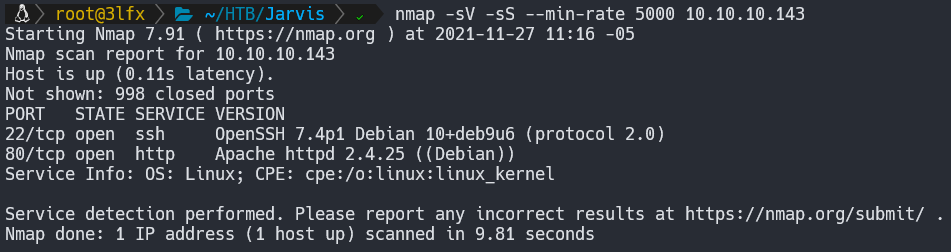
\includegraphics[width=0.99\textwidth]{imagenes/jarvis/01_nmap_jarvis.png}
            \caption{Escaneo de puertos Jarvis} 
        \end{figure}  

    \subsubsection{Análisis de Vulnerabilidades}

        \large{Al analizar el servicio web, se encontro una página web relacionada a un hotel.}
        \par
        \begin{figure}[H]
            \centering
            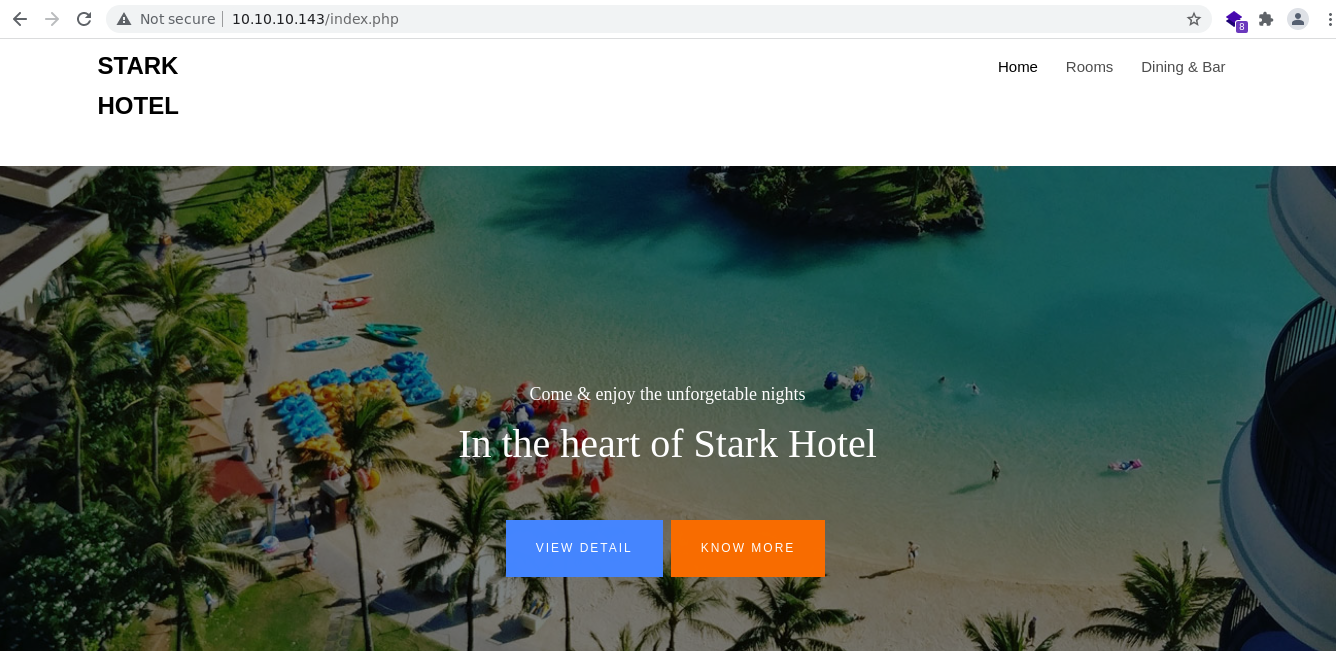
\includegraphics[width=0.99\textwidth]{imagenes/jarvis/02_index_jarvis.png}
            \caption{Página Web Jarvis}
        \end{figure}

        \large{Lo siguiente a realizar fue usar la herramienta "Gobuster" para enumerar los directorios de la página web.}
        \par
        \begin{figure}[H]
            \centering
            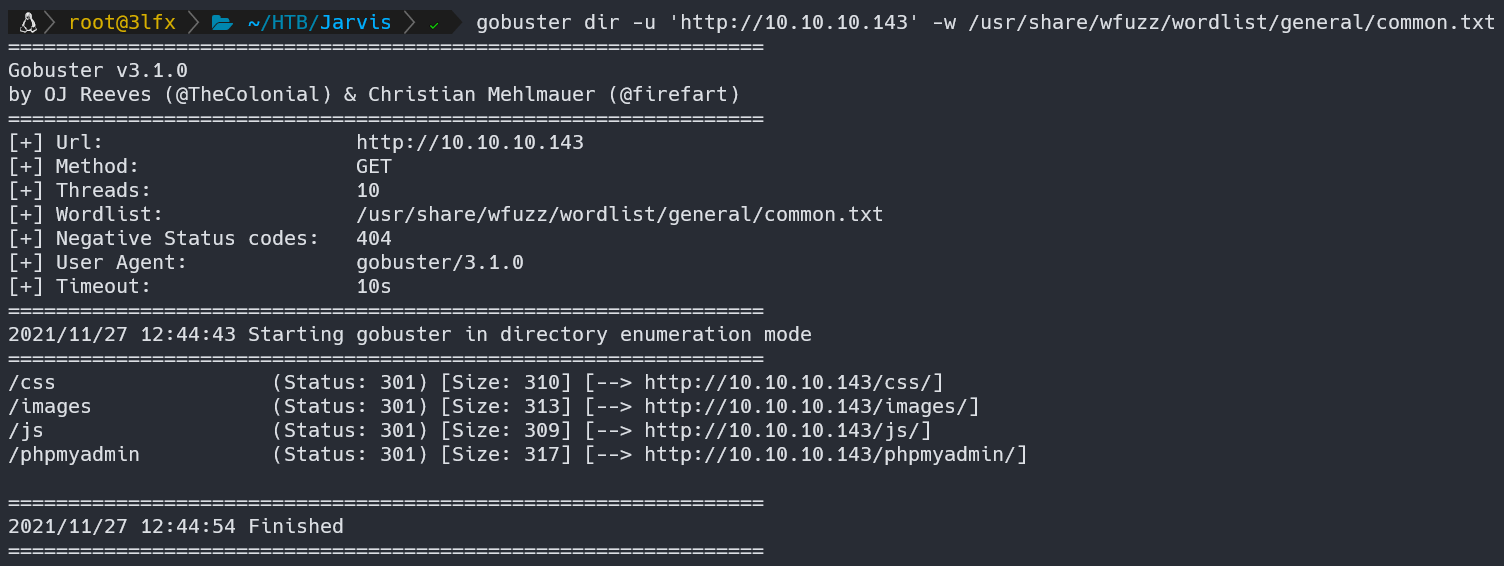
\includegraphics[width=0.99\textwidth]{imagenes/jarvis/03_gobuster_jarvis.png}
            \caption{Enumeración de directorios en Jarvis}
        \end{figure}
        
        \large{Del paso anterior se registró 4 directorios, siendo los 3 primeros directorios comunes, se procedió a acceder al último "/phpmyadmin", donde se encontraba una Login al gestor de la base de datos de Jarvis.}
        \par
        \begin{figure}[H]
            \centering
            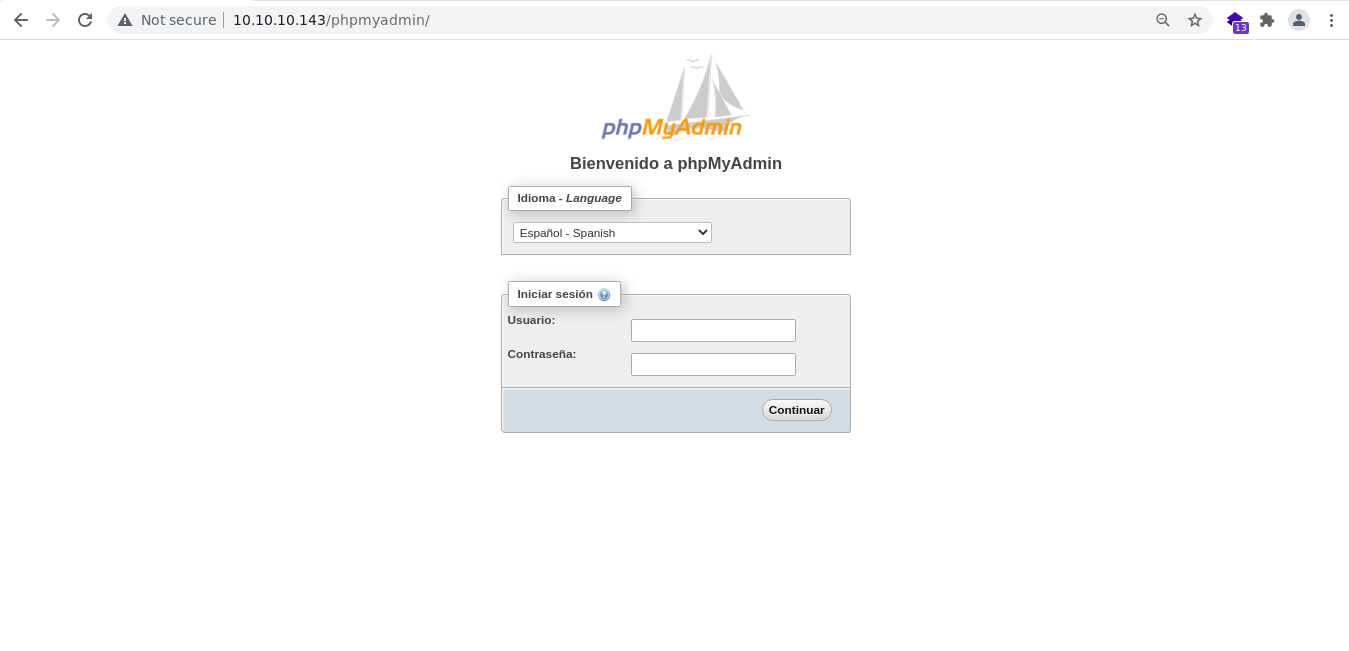
\includegraphics[width=0.99\textwidth]{imagenes/jarvis/04_phpmyadmin_jarvis.png}
            \caption{Login a phpMyAdmin en Jarvis}
        \end{figure}

        \large{Al buscar información sobre la versión de este servicio, se encontró que tiene una vulnerabilidad de inclusión de archivos remotos (CVE-2018-12613), para la cual existe un exploit.}
        \par
        \begin{figure}[H]
            \centering
            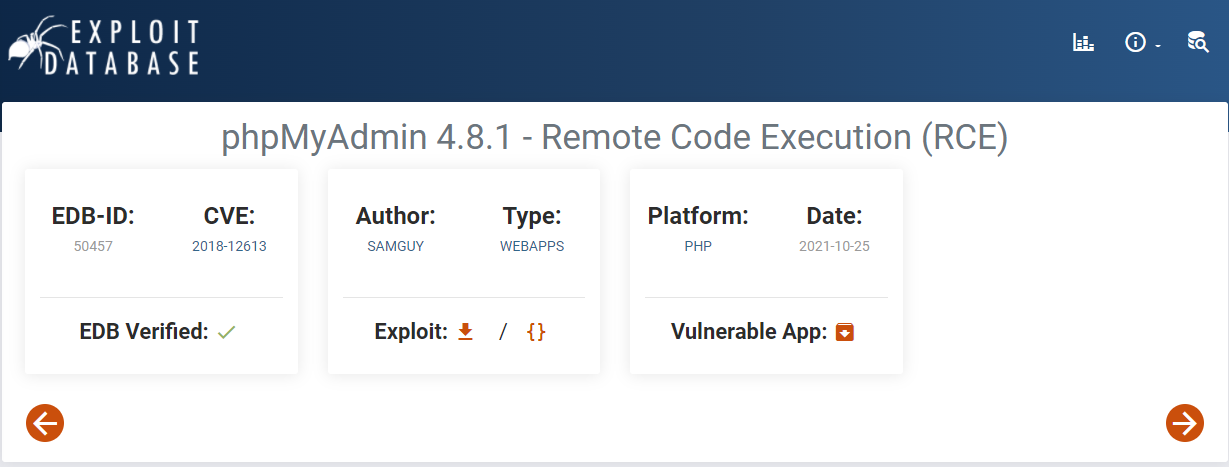
\includegraphics[width=0.99\textwidth]{imagenes/jarvis/05_exploitdb_jarvis.png}
            \caption{Exploit para phpMyAdmin 4.8.1 en Jarvis}
        \end{figure}

        \large{Para poder explotar la vulnerabilidad con el exploit, se intento acceder al Login con las credenciales comunes, al o funcionar se continuo revisando la página web donde se encontró una sección de habitaciones.}
        \par
        \begin{figure}[H]
            \centering
            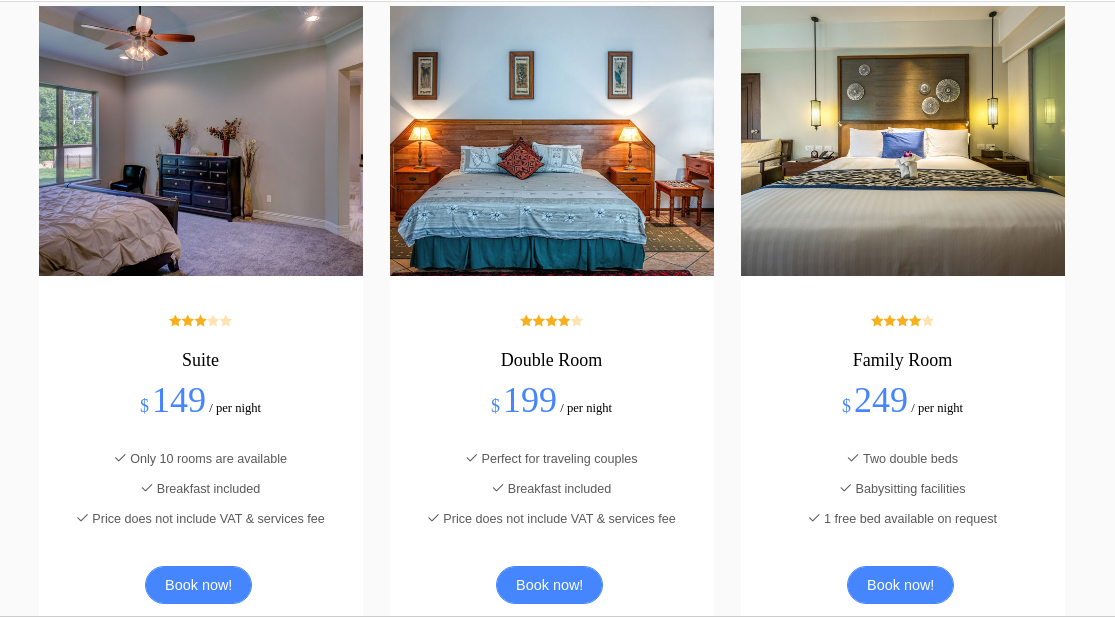
\includegraphics[width=0.99\textwidth]{imagenes/jarvis/06_seccion_rooms_jarvis.png}
            \caption{Sección de habitaciones en Jarvis}
        \end{figure}

        \large{Al acceder a cada una de estas, se pudo observar que la dirección de la web cambió y que se proporcionaba un codigo por cada habitación.}
        \par
        \begin{figure}[H]
            \centering
            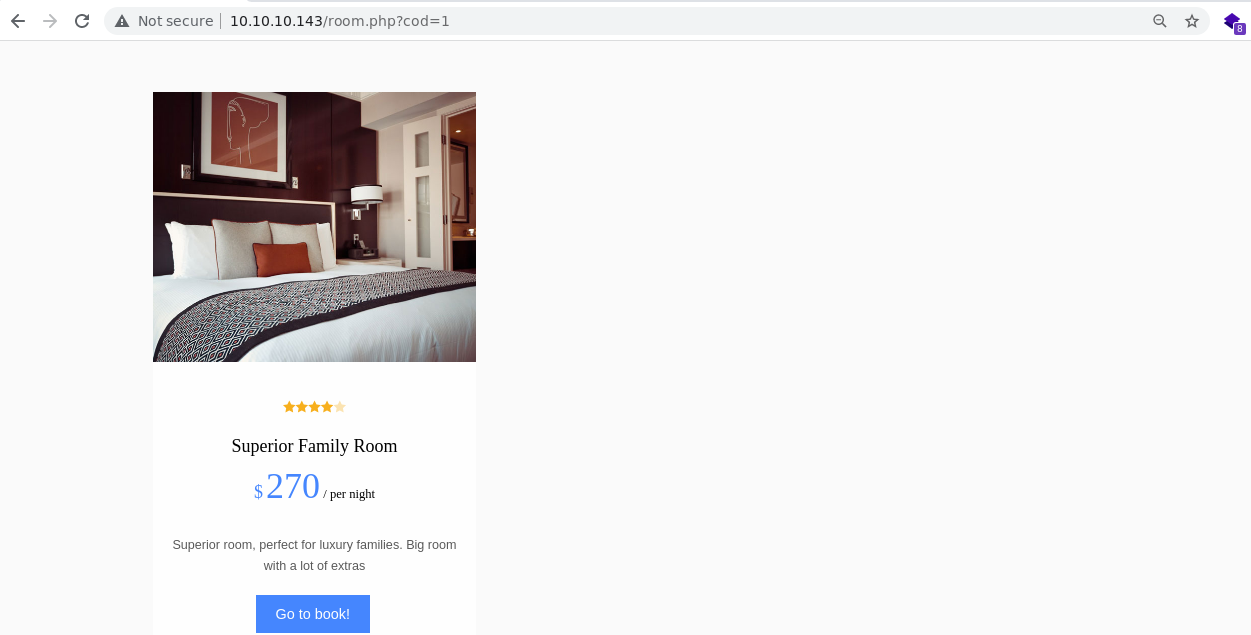
\includegraphics[width=0.99\textwidth]{imagenes/jarvis/07_room_jarvis.png}
            \caption{Interfaz de una habitación en Jarvis}
        \end{figure}

        \large{Utilizamos esa nueva direción para aplicar la injección de sql con la herramienta "sqlmap".}
        \par
        \begin{figure}[H]
            \centering
            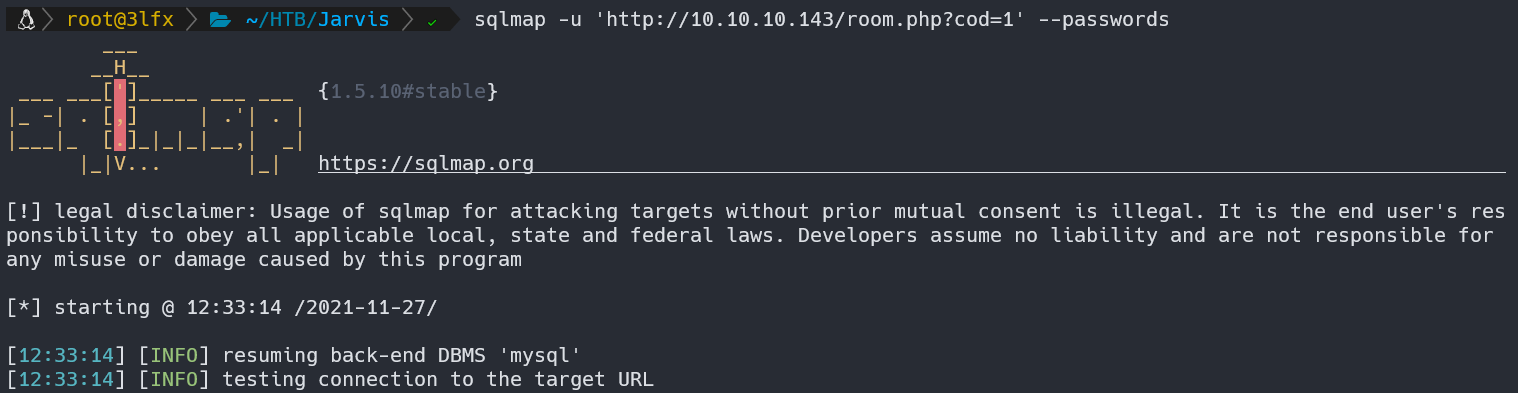
\includegraphics[width=0.99\textwidth]{imagenes/jarvis/08_sql_map_jarvis.png}
            \caption{Ejecución de sqlmap en Jarvis}
        \end{figure}

        \large{Con el "sqlmap" logramos obtener el usuario (DBadmin) y la contraseña (imissyou) del Login.}
        \par
        \begin{figure}[H]
            \centering
            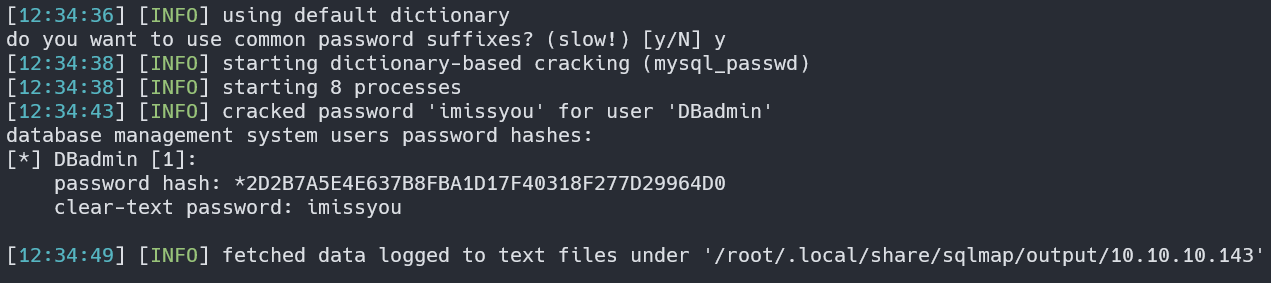
\includegraphics[width=0.99\textwidth]{imagenes/jarvis/09_db_pass_jarvis.png}
            \caption{Credenciales del Login de phpMyAdmin en Jarvis}
        \end{figure}

    \subsubsection{Explotación}

        \large{Utilizamos las credenciales para acceder al Login.}
        \par
        \begin{figure}[H]
            \centering
            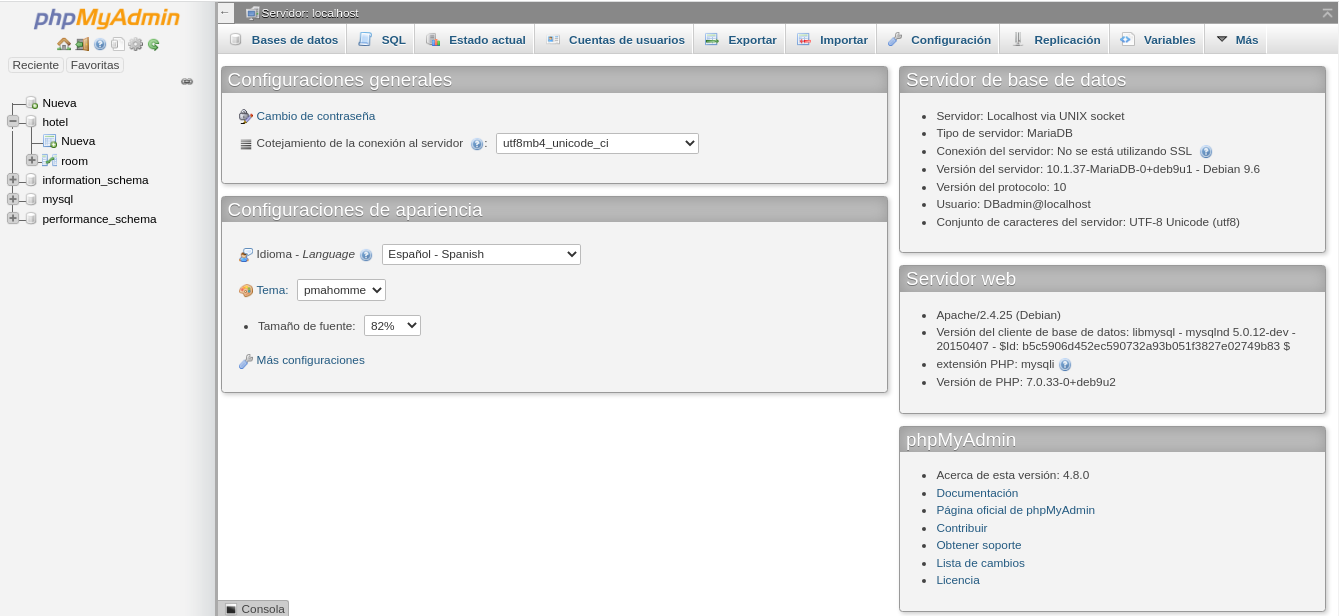
\includegraphics[width=0.99\textwidth]{imagenes/jarvis/10_phpmyadmin_dentro_jarvis.png}
            \caption{Dentro de phpMyAdmin en Jarvis}
        \end{figure}

        \large{Con el acceso obtenido, se puede revisar la información del phpMyAdmin y se procedio a ejecutar el exploit, para ello primero se descargo y luego ejecutado, brindando la ip de la máquina atacante y el puerto de escucha.}
        \par
        \begin{figure}[H]
            \centering
            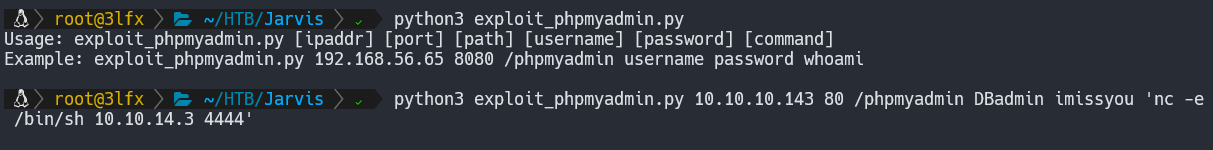
\includegraphics[width=0.99\textwidth]{imagenes/jarvis/11_exploit_phpmyadmin_jarvis.png}
            \caption{Ejecución del Exploit en Jarvis}
        \end{figure}

        \large{Ya habiendo ejecutado el exploit, utilizamos reverse shell para tener control de la máquina objetivo, ya en la máquina ejecutamos el comando "whoami", el cual nos brinda el nombre de usuario asociado con la identificación de usuario efectiva actual de esta máquina, el cual es "www-data".}
        \par
        \begin{figure}[H]
            \centering
            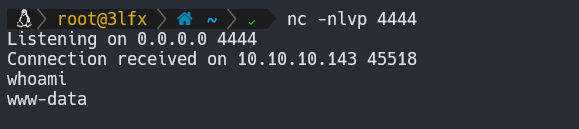
\includegraphics[width=0.99\textwidth]{imagenes/jarvis/12_reverse_shell_jarvis.png}
            \caption{Reverse shell en Jarvis}
        \end{figure}

    \subsubsection{Escalamiento de Privilegios}

        \large{Con el usuario www-data ejecutamos el comando "sudo -l" para obtener los permisos que posee, como se aprecia en la imagen de abajo}
        \par
        \begin{figure}[H]
            \centering
            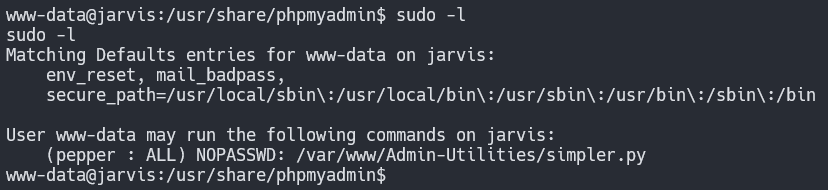
\includegraphics[width=0.99\textwidth]{imagenes/jarvis/13_permiso_www_jarvis.png}
            \caption{Permisos de "www-data" en Jarvis}
        \end{figure}

        \large{Se identificó que el nombre de usuario de la máquina es "pepper" y tiene acceso a un archivo python llamado "simpler.py", el cual ejecutamos, como de aprecia en la siguiente imagen.}
        \par
        \begin{figure}[H]
            \centering
            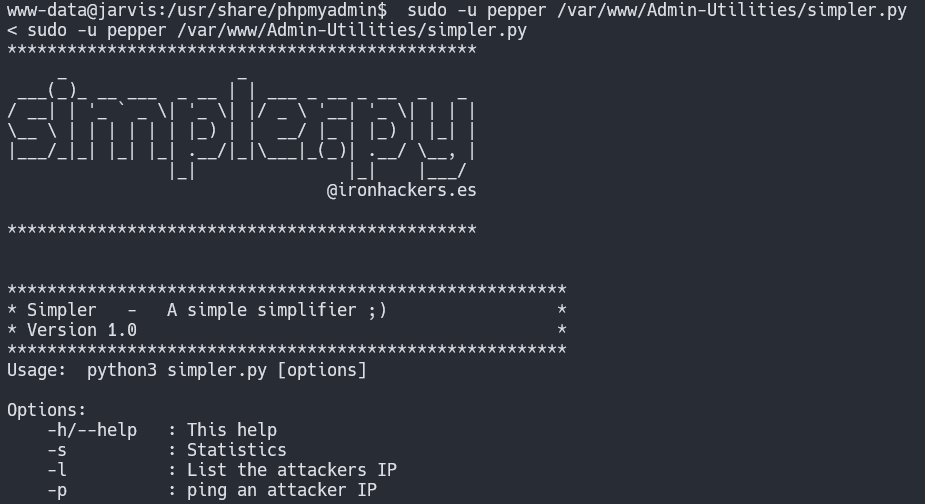
\includegraphics[width=0.99\textwidth]{imagenes/jarvis/14_simpler_python_jarvis.png}
            \caption{Ejecución de "Simpler.py" en Jarvis}
        \end{figure}

        \large{En el código python ejecutado se encuentra la función que se aprecia en la imagen de abajo, la cual nos dice que mientras no se usen los carácteres listados no terminará la ejecucuón del código.}
        \par
        \begin{figure}[H]
            \centering
            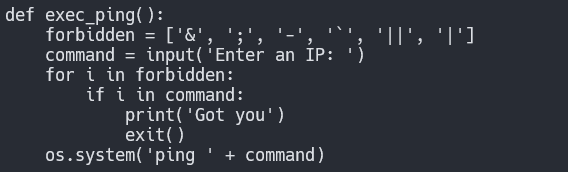
\includegraphics[width=0.99\textwidth]{imagenes/jarvis/15_fun_ping_jarvis.png}
            \caption{Función de Simpler.py en Jarvis}
        \end{figure}

        \large{Probamos ejecutar el comando bash con el carácter especial de dolár, pues no se encuentra en la lista mencionada previamente.}
        \par
        \begin{figure}[H]
            \centering
            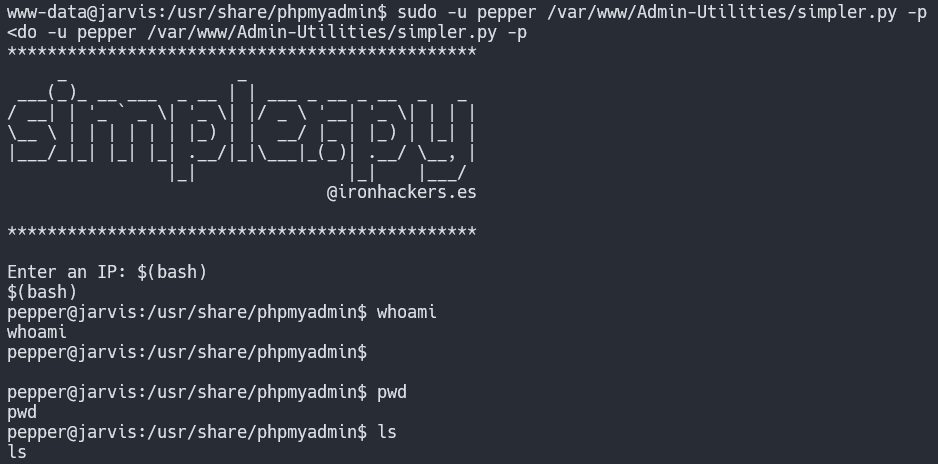
\includegraphics[width=0.99\textwidth]{imagenes/jarvis/16_prueba_bash_jarvis.png}
            \caption{Prueba del comando "bash" en Jarvis}
        \end{figure}

        \large{Ahora, con la información obtenida por el bash aplicamos reverse shell al usuario "peppers".}
        \par
        \begin{figure}[H]
            \centering
            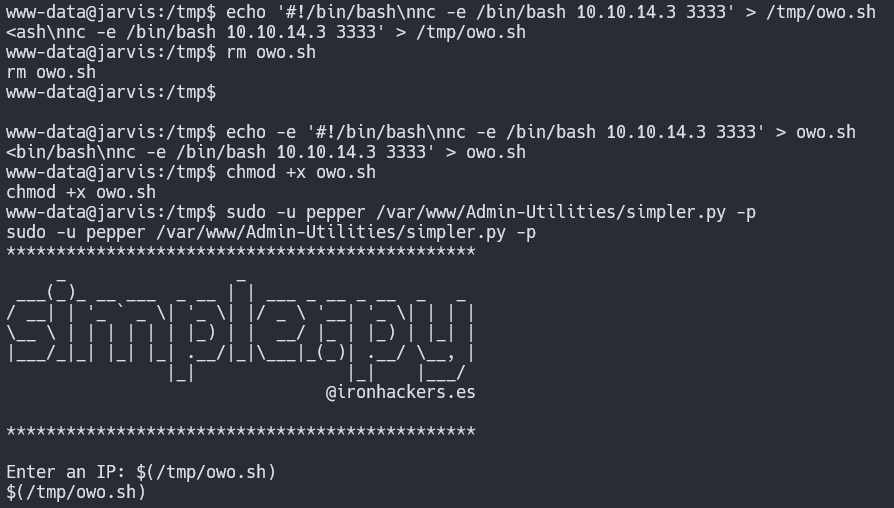
\includegraphics[width=0.99\textwidth]{imagenes/jarvis/17_reverse_peppers_jarvis.png}
            \caption{Aplicación de Reverse shell a "peppers" en Jarvis}
        \end{figure}

        \large{Abrimos el puerto de escucha en la máquina atacante y verificamos que estemos con el usuario correcto.}
        \par
        \begin{figure}[H]
            \centering
            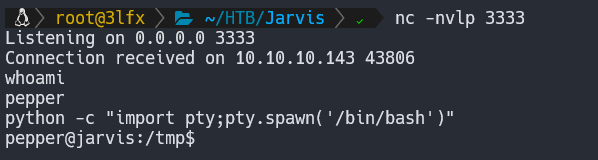
\includegraphics[width=0.99\textwidth]{imagenes/jarvis/18_conect_peppers_jarvis.png}
            \caption{Conexión a "peppers" en Jarvis}
        \end{figure}

        \large{Ya con el usuario "peppers" revisando los archivos que contiene, encontramos un user.text donde se ubica la flag del usuario.}
        \par
        \begin{figure}[H]
            \centering
            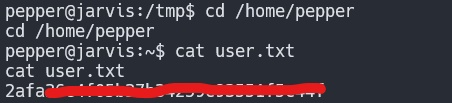
\includegraphics[width=0.99\textwidth]{imagenes/jarvis/19_user_flag_jarvis.jpg}
            \caption{User flag de Jarvis}
        \end{figure}

        \large{Ahora tratamos de escalar privilegios en la máquina, para ello listamos los archivos binarios con permiso SUID, como se aprecia en la siguiente imagen.}
        \par
        \begin{figure}[H]
            \centering
            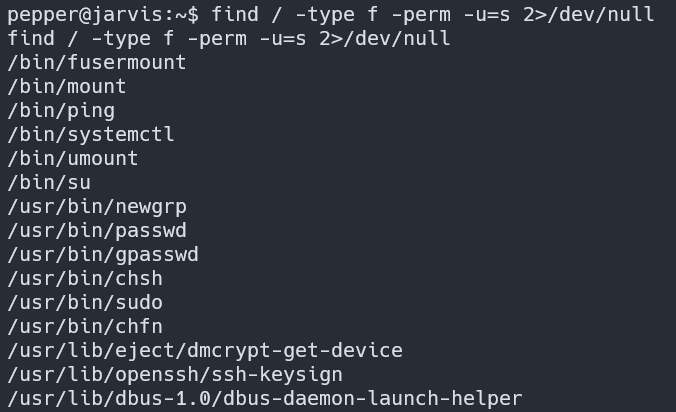
\includegraphics[width=0.99\textwidth]{imagenes/jarvis/20_binarios_suid_jarvis.png}
            \caption{Archivos binarios en Jarvis}
        \end{figure}

        \large{Con los archivos listados, buscamos el que proporcione la información de los accesos de root de la página, de acuerdo a la siguiente documentación encontrada.}
        \par
        \begin{figure}[H]
            \centering
            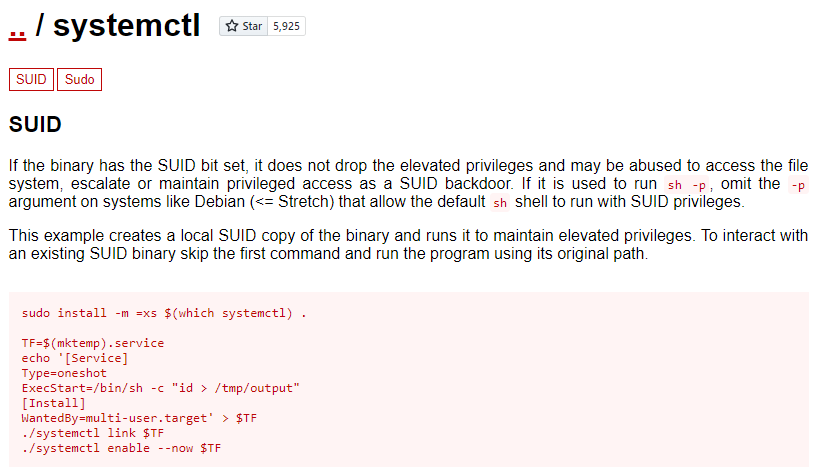
\includegraphics[width=0.99\textwidth]{imagenes/jarvis/21_systemctl.png}
            \caption{Systemctl}
        \end{figure}

        \large{Utilizamos el servicio reverse de la siguiente manera.}
        \par
        \begin{figure}[H]
            \centering
            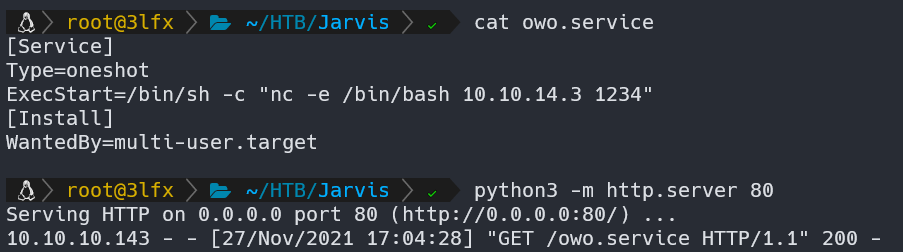
\includegraphics[width=0.99\textwidth]{imagenes/jarvis/22_servicio_reverse_jarvis.png}
            \caption{Servicio reverse en Jarvis}
        \end{figure}

        \large{Procedemos a descagar el reverse.}
        \par
        \begin{figure}[H]
            \centering
            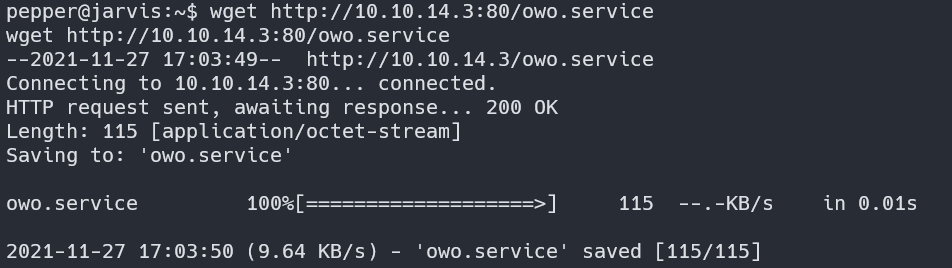
\includegraphics[width=0.99\textwidth]{imagenes/jarvis/23_descarga_reverse_jarvis.png}
            \caption{Servicio reverse en Jarvis}
        \end{figure}

        \large{Y ahora lo ejecutamos.}
        \par
        \begin{figure}[H]
            \centering
            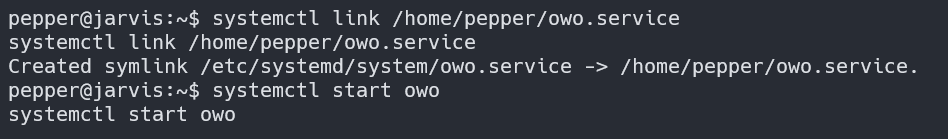
\includegraphics[width=0.99\textwidth]{imagenes/jarvis/24_ejecu_servicio.png}
            \caption{Servicio reverse en Jarvis}
        \end{figure}

        \large{Establecemos el puerto de escucha y se puede verificar que se consiguió el acceso a root.}
        \par
        \begin{figure}[H]
            \centering
            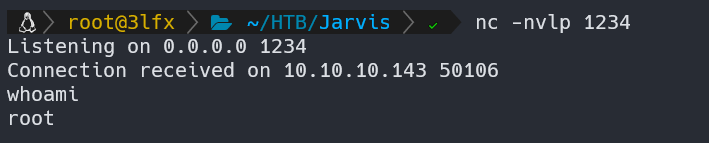
\includegraphics[width=0.99\textwidth]{imagenes/jarvis/25_conect_root_jarvis.png}
            \caption{Conexión a root en Jarvis}
        \end{figure}

        \large{Revisando los archivos del usuario root, encontramos el archivo "root.txt" con su respectiva flag.}
        \par
        \begin{figure}[H]
            \centering
            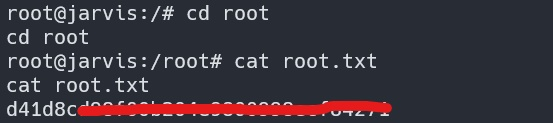
\includegraphics[width=0.99\textwidth]{imagenes/jarvis/26_root_flag_jarvis.jpg}
            \caption{Root flag en Jarvis}
        \end{figure}

    \subsubsection{Post-Explotación}

        \large{Se crea una carpeta ".ssh" para almacenar la llave pública de Jarvis.}
        \par
        \begin{figure}[H]
            \centering
            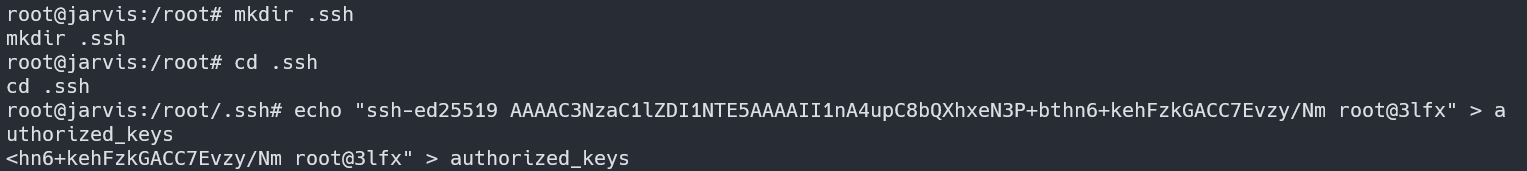
\includegraphics[width=0.99\textwidth]{imagenes/jarvis/27_public_key_jarvis.png}
            \caption{Carpeta ".ssh" y llave pública en Jarvis}
        \end{figure}

        \large{Especificamos las claves para el ssh como se muestra abajo.}
        \par
        \begin{figure}[H]
            \centering
            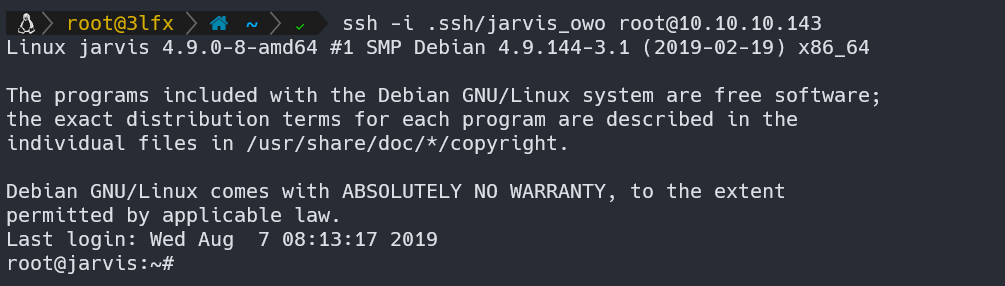
\includegraphics[width=0.99\textwidth]{imagenes/jarvis/28_ssh_root_jarvis.png}
            \caption{Claves root en Jarvis}
        \end{figure}

        \large{Para terminar esta fase, se procede a extraer ña credenciales de los usuarios de la máquina Jarvis.}
        \par
        \begin{figure}[H]
            \centering
            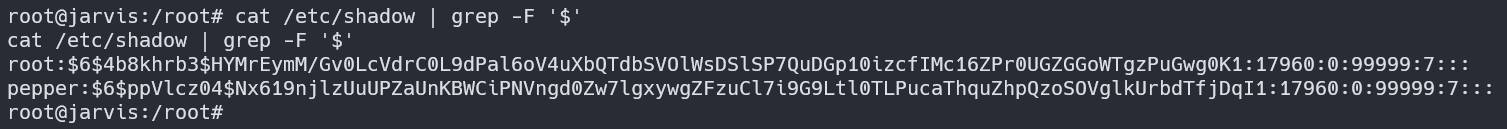
\includegraphics[width=0.99\textwidth]{imagenes/jarvis/29_hashes_jarvis.png}
            \caption{Extracción de contraseñas en formato hash de Jarvis}
        \end{figure}

    \subsubsection{Recomendaciones de Mitigación}

    \subsection{HTB02 - Time}
    \subsection{HTB03 - Forest}
    \subsubsection{Escaneo}
        \large{Como inicio de la prueba de penetración se realiza un escaneo de puertos con la herramienta "Nmap", donde se encuentran once puertos abiertos.}
        \par
        \begin{figure}[h!]
            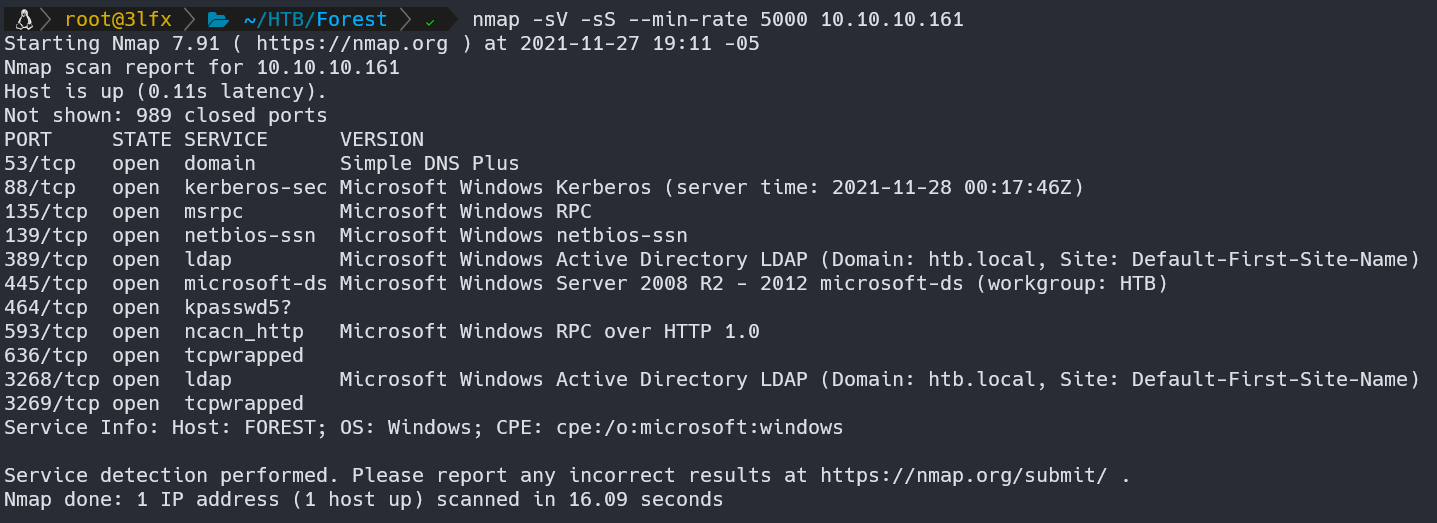
\includegraphics[width=1\textwidth]{imagenes/nmap_forest.png} \par \vspace{0.1cm}
            \caption{Escaneo de puertos Forest} 
        \end{figure}
    \subsubsection{Análisis de vulnerabilidades y debilidades}
    
    \clearpage
%------Conclusiones-----------
\end{document}